\documentclass[9pt,twoside]{pnas-new}

\templatetype{pnasmathematics} 

\usepackage{subfigure}

\title{Github Collaborator Recommendation}

% Authors should be listed in alphabetical order by last name. Use letters to indicate affiliations.
\author[a]{Albert Jian} 
\author[a]{Bill Wen}
\author[a]{Shan Zhong}

\affil[a]{University of California, Los Angeles}

% Please give the surname of the lead author for the running footer
\leadauthor{Zhong, Jian, Wen} 

% Please add a significance statement to explain the relevance of your work
\significancestatement{Recommender system in social network aims to predict the most probable hidden friendship within the network and recommend it to the users. In this paper, we use network theory feature to develop machine learning model for a recommender system and analyzes the importance of different features within the model.}

% Please include author contributions here.
\authorcontributions{}

% Please provide three to five keywords, separated by the pipe symbol. Keywords will signal the application, methods, etc. to the reader.
\keywords{Machine Learning $|$ Recommender System $|$ Social Networks } 

\begin{abstract}
Recommender systems in the context of social networks recommends a likely acquaintance to a user. In this paper, we use concepts from network theory to develop features for machine learning to produce a recommender system to suggest GitHub followees to users. Using training and testing sets, we are able to demonstrate highly accurate recommender system using machine learning models. From the result, we found that the most important features are personalized PageRank scores, and how similar is the suggested followee to the current user's followees.
\end{abstract}

\dates{This manuscript was compiled on \today}
\doi{Math 168 Spring 2020 Final Project}

\begin{document}

\maketitle
\thispagestyle{firststyle}
\ifthenelse{\boolean{shortarticle}}{\ifthenelse{\boolean{singlecolumn}}{\abscontentformatted}{\abscontent}}{}

% If your first paragraph (i.e. with the \dropcap) contains a list environment (quote, quotation, theorem, definition, enumerate, itemize...), the line after the list may have some extra indentation. If this is the case, add \parshape=0 to the end of the list environment.
\dropcap{D}uring the recent rise of web services, many companies utilize different version of recommender system to recommend personalized items to their users, including Google's infamous YouTube algorithm. In social networks, recommender system recommend the more probable connections to the user. 

In this paper we produce a recommendation system for a GitHub social network using machine learning approaches. We will first analyze our results and discuss their relevance, then we will describe the dataset and concepts from network theory and machine learning we used to develop the recommender system.

\section*{Results}

\begin{table}[th]
    \centering
    \caption{Model Hyperparameters and Training and Testing F\textsubscript{1} Score}
    \begin{tabular}{lrrr}
    Model & Hyperparameters(max\_depth, n\_estimators) & Train F\textsubscript{1} & Test F\textsubscript{1} \\
    \midrule
    Random Forest & (14, 121) & 0.96 & 0.92 \\
    Gradient Boosting Decision Tree & (10, 200) & 0.99 & 0.99 \\
    \bottomrule
    \end{tabular}
\end{table}   

\section*{Discussion}

\section*{Materials}
\subsection*{Dataset}
The dataset GitHub Social Network is taken from SNAP \cite{rozemberczki2019multiscale}. This dataset contains a large social network of GitHub developers collected from the public API in June 2019. Nodes are developers who have starred at least 10 repositories and edges are mutual follower relationships between them. The dataset consists of 37700 nodes and 289003 edges.
\subsection*{Exploratory Data Analysis}
The degree distribution of the network is shown in figure \ref{fig:follows}. The largest number of mutual follows is 9458 and the minimum number is 1. 5045 users in the network have 1 mutual follow and around 25000 people have less than 5 mutual follows. As seen from both of the graphs, the degree distribution is quite left-skewed. 

In order to visualize the network, we picked a central node from the training set and we performed a breadth-first walk of the group to a maximum distance of 3 as shown in figure \ref{fig:localnetwork}. Nodes are sized according to their distance from the center and colored by their personalized PageRank with the central node.

\begin{figure}[th]
    \centering
    \subfigure[Mutual follows for the least 30000 users]{
        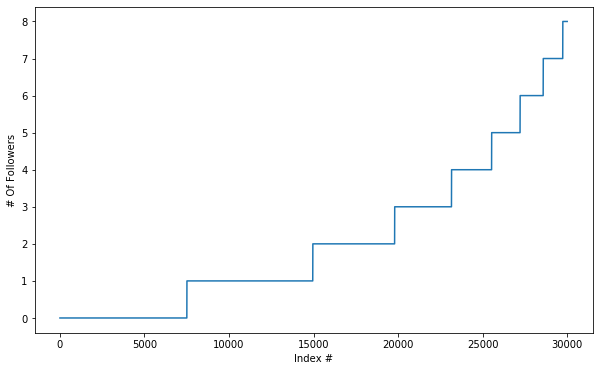
\includegraphics[width=0.4\textwidth]{Figures/followers_30000.png}
    }
    \subfigure[Mutual follows box plot]{
        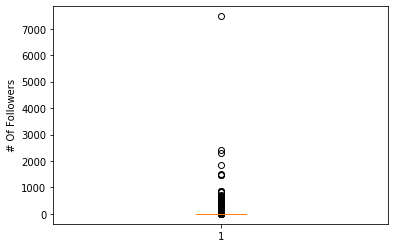
\includegraphics[width=0.4\textwidth]{Figures/followers_boxplot.png}
    }
    \caption{Mutual follows per user}
    \label{fig:follows}
\end{figure}

\begin{figure}[ht]
    \centering
    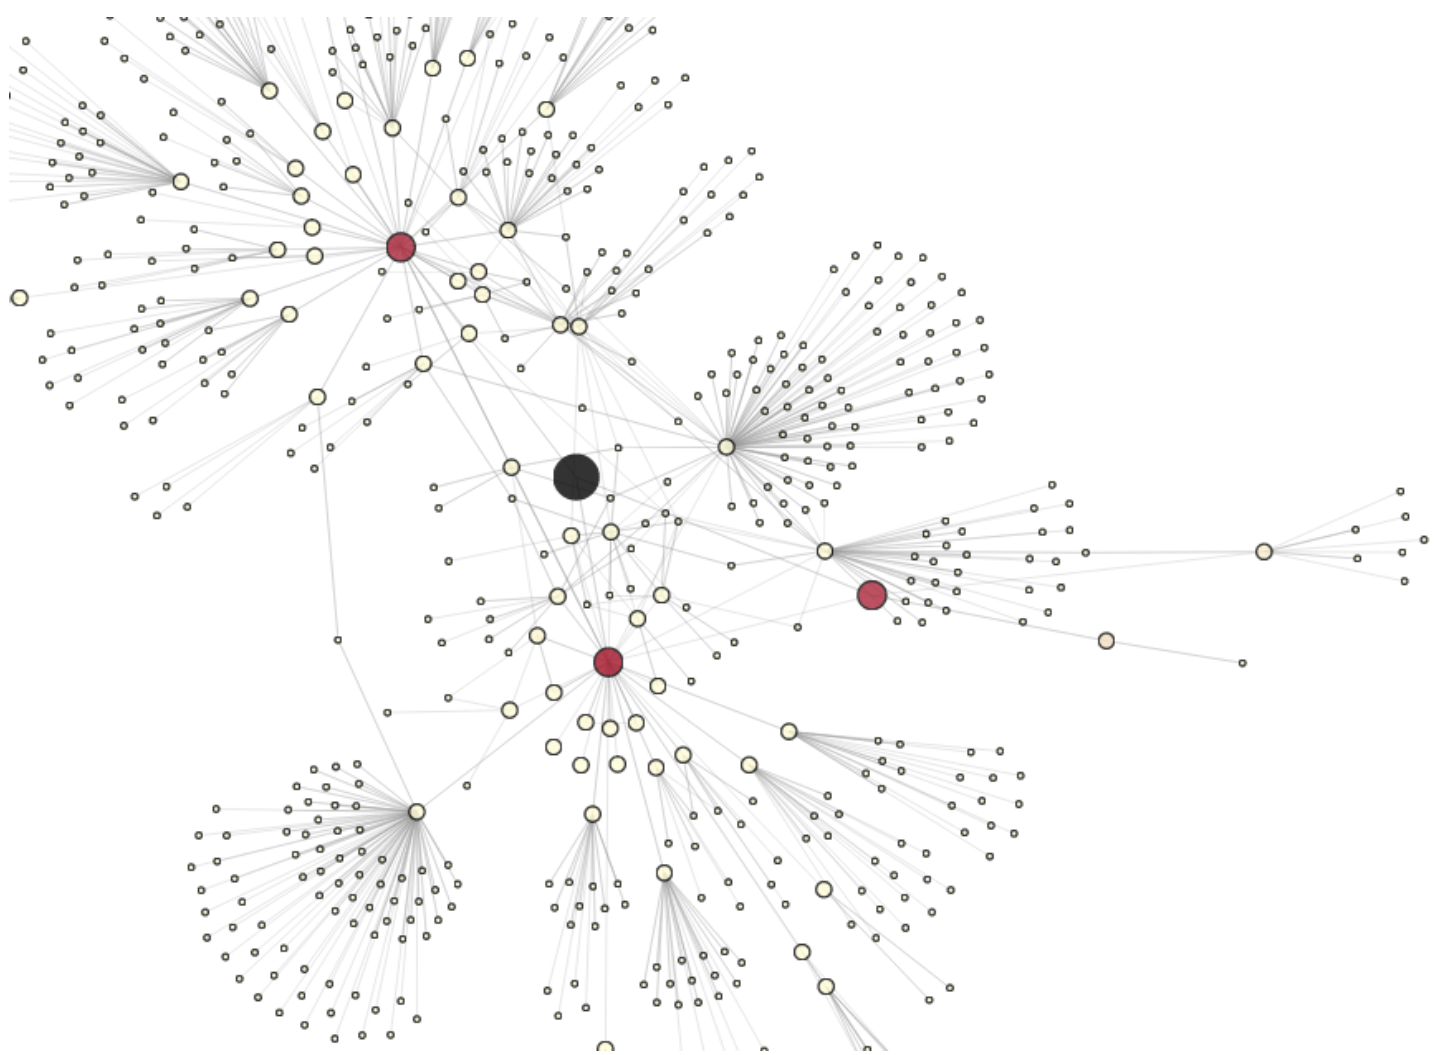
\includegraphics[width=0.5\textwidth]{Figures/local_network_example.png}
    \caption{Example Local Network with Distance of 3}
    \label{fig:localnetwork}
\end{figure}


\section*{Methods}
The methods in this paper is mostly inspired by this research in link prediction in social networks \cite{6033365}. Binary classification method (Random Forest, Support Vector Machine and Gradient Boosting) was adopted to classify good links and bad links. SVD was applied to reduce the dimension of the dataset. Similarity measures such as jaccard distance, cosine distance and preferential attachment were calculated as features. Ranking measures (page rank), centrality measures (Katz centrality) and other metrics such as shortest path and common neighbors were also added for model training. Confusion matrix was plotted at the end to evaluate model performance. We trained for two separate models, one with Random Forest, RF, and one with Gradient Boosting Decision Tree, GBDT. 
\subsection*{Features}\cite{sadraei}

\subsubsection*{Jaccard's Coefficient}

\subsubsection*{Preferential Attachment}

\subsection*{Machine Learning Models}


\acknow{We would like to acknowledge our professor Dr. Heather Zinn-Brooks and our teaching assistant Abigail Hickok for their accomodations during the remote instructions this quarter.}

\showacknow % Display the acknowledgements section

% Bibliography
\bibliography{References}

\end{document}
